\documentclass[11pt, oneside]{article}   	% use "amsart" instead of "article" for AMSLaTeX format
\usepackage{geometry}                		% See geometry.pdf to learn the layout options. There are lots.
\geometry{letterpaper}                   		% ... or a4paper or a5paper or ... 
%\geometry{landscape}                		% Activate for for rotated page geometry
%\usepackage[parfill]{parskip}    		% Activate to begin paragraphs with an empty line rather than an indent
\usepackage{graphicx}				% Use pdf, png, jpg, or eps§ with pdflatex; use eps in DVI mode
								% TeX will automatically convert eps --> pdf in pdflatex		
\usepackage{amssymb}
\usepackage{amsmath}
\usepackage{float}

\title{Analysis on Popular Language Models}
%\author{R02944047 R03922141}
%\date{}							% Activate to display a given date or no date

\begin{document}
\maketitle
\section{Introduction}
A statistical language model is a probability distribution over sequences of words. It can be used in many natural language processing applications such as speech recognition, machine translation and information retrieval, by estimating the relative likelihood of different phrases. Researchers have derived many reasonable language models, and some of those models are quite classical and popular nowadays. In the following sections, we will introduce the knowledge of N-gram model, Neural Network language model, Recurrent Neural Network language model and Skip-gram model, and analyse their characteristics both in theory and practice.
\subsection{N-gram Model}
In an n-gram model$^{[1]}$, given an sequence $(w_1,w_2,...,w_m)$, which is assumed as a Markov chain, the probability of observing the sequence is defined as:
\[
P(w_1,w_2,...,w_m)=\prod_{i=1}^{m}{P(w_i|w_1,w_2,...,w_{i-1})}= \prod_{i=1}^{m}{P(w_i|w_{i-(n-1)}...,w_{i-1})}.
\]
The conditional probability can be calculated from n-gram frequency:
\[
P(w_i|w_{i-(n-1)}...,w_{i-1})=\frac{\text{count}(w_{i-(n-1)}...,w_{i-1},w_{i})}{\text{count}(w_{i-(n-1)}...,w_{i-1})}.
\]
In addition, some smoothing methods such as Good Turing, and back-off strategies like Katz are used to deal with out-of-vocabulary words, which help to build a more sophisticated model.

\subsection{Neural Network Language Model}
A neural network language model(NNLM) also computes the conditional probability of a n-gram, while it uses neural network to estimate a vector representation of each word. The most contributive model was suggested by Y. Bengio's et al.$^{[2]}$. Figure 1 shows its architecture. It finds a good way to make similar word closer in vector space.
\begin{figure}
\centering
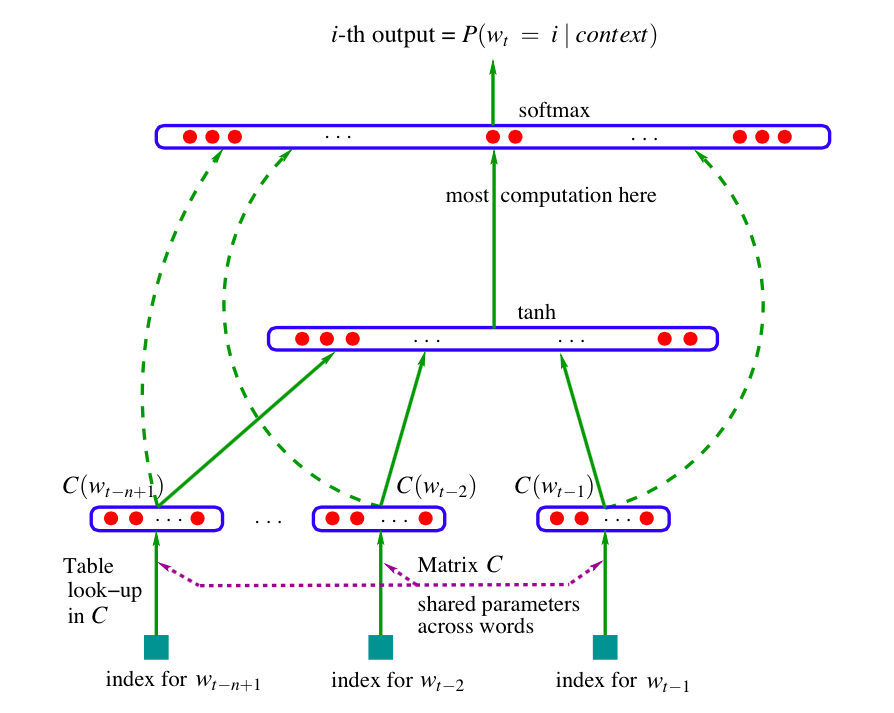
\includegraphics[width=250pt]{nnlm.png}
\caption{Architecture of NNLM, where $C(i)$ is the $i$-th word feature vector}
\end{figure}
The general feedforward procedure of the neural network can be described as follows: 
\begin{enumerate}
\item Assign a $M \times 1$ vector $C(w_i)$ to represent a word $w_i$
\item Project the concatenation of vectors $[C(w_{t-n+1}),...,C(w_{t-1})]$ to the hidden layer. The projection function is like:
\[z=W_1C(w_{t-n+1}) + ... + W_{n-1}C(w_{t-1}),
\] where  $W_i$ is a $H\times M$ matrix.
\item Apply an activation function $h=f(z)$ such as tanh, sigmoid in the hidden layer.
\item Project  vector $h$ by $s=W_hh$ to the output layer, where $W_h$ is a $V\times H$ matrix, $V$ is the size of the vocabulary.
\item Apply softmax function $O=\text{softmax}(s)$, thus $O_j =P(w_t=j|\text{context})$, where $j$ is the word index in the vocabulary. 
\end{enumerate}
And the produce of the back-propagation can be describe as follows:
\begin{enumerate}
\item Define the loss function $L(s,h,W_h,z,W,C)=-log(O_j)$ 
\item Compute the sub-gradient of L for each variable backward the network.
\item Update parameters $W_h,W$ and input vector $C$ according to gradient descent algorithm.
\end{enumerate}

\subsection{Recurrent Neural Network Language Model}

Similar as NNLM, the Recurrent Neural Network Language Model(RNNLM)$^{[3]}$ also use a vector to represent a word and compute conditional probability of each word according to the context. However, other than using n-gram framework, RNN takes whole context into consideration. The architecture of RNNLM is shown in Figure 2.

\begin{figure}[H]
\centering
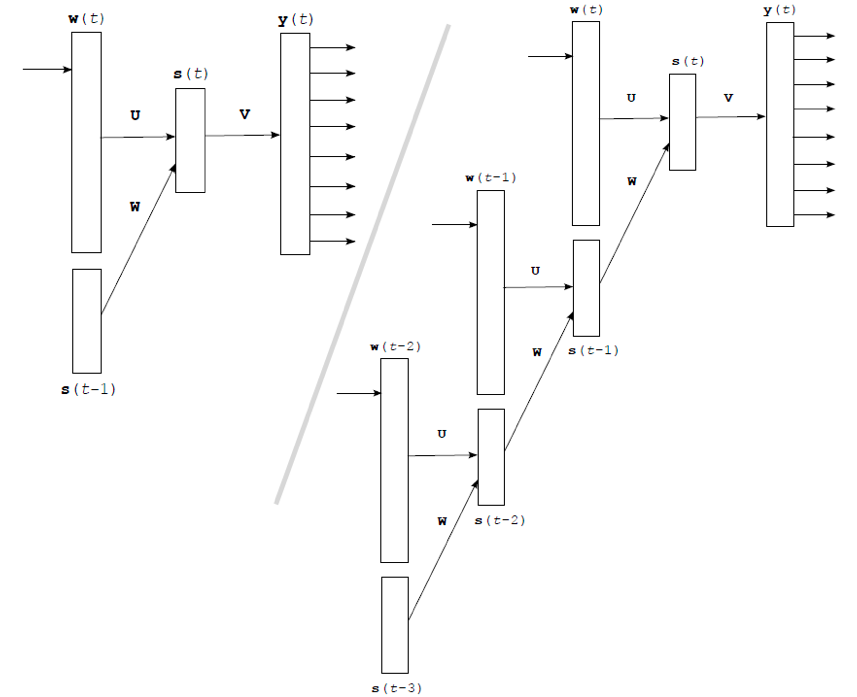
\includegraphics[width=250pt]{rnnlm.png}
\caption{Architecture of RNNLM, the left side shows the forward phase and the right side shows the backward phase.}
\end{figure}
The input layer consists of a vector $w(t)$ that represents the current word, and vector $s(t-1)$ represents output values in the hidden layer from the previous time step. The output layer $y(t)$ represents the conditional probability $P(w_{t+1}|w_t, s(t-1)). $ And the output values in the hidden layer and output layer are computed as follows: 
\[
s(t)=f(Uw(t)+Ws(t-t))
\]
\[
y(t)=g(Vs(t))
\]
where, $f(z)$ and $g(z)$ are sigmoid and softmax functions, $U,W,V$ are projection matrices between input, hidden and output layers. 
The time complexity of one training or test step is proportional to :
\[
O=H\times H + H\times V = H(H+V)
\]
where H is size of the hidden layer and V is size of the vocabulary. \\

RNNLM is trained by stochastic gradient descent using either usual backpropagation (BP) algorithm, or backpropagation through time (BPTT). The objective function that we aim to maximize is likelihood of the training data:
\[
f(\lambda)=\sum_{t=1}^{T}logy_{l_{t}}(t),
\]
where $l_t$ is the index of the correct predicted word for the $t$-th sample. And the parameters can be updated as:
\[
V(t+1)=V(t)+s(t)e_o(t)^T\alpha-V(t)\beta
\]
\[
U(t+1)=U(t)+w(t)e_h(t)^T\alpha-U(t)\beta
\]
\[
W(t+1)=W(t)+s(t-1)e_h(t)^T\alpha-W(t)\beta
\]
where $e_o$ and $e_h$ are the error gradient of the output and hidden layer,  $\alpha$ is the learning rate and $\beta$ is the regularization parameter.

\subsection{Skip-gram and Word2vec}
A Skip-gram$^{[4]}$ model is to some degree like a varied and efficient version of NNLM which using skip-gram instead of traditional n-gram. A k-skip-n-gram for a sentence  $(w_1,w_2,...,w_m)$ is defined as:
\[
\{w_{i_1},w_{i_2},...,w_{i_n}|\sum_{j=1}^{n}{i_j-i_j-1} <k\}
\]
And Word2vec$^[5]$ is a tool that provides an efficient implementation of the continuous bag-of-words and skip-gram architectures for computing vector representations of words.
\section{Experiment}
\subsection{Evaluation}
Since language model prefers sentences that are more frequently observed and grammatical, a reasonable way to evaluate a language model is to test whether it will pick real sentence out of some random generated sentence. So we evaluate the performances of the above language models by completing an open shared task for language modelling in [6].

The task is to assign scores to sentences, based on their quality. The dataset contains 10,000 sentences that need to be scored. The sentences are in pairs - one correct and one incorrect sentence. The paired sentences are kept together in the dataset, but it is randomly selected whether the correct sentence is first or second. The "unk10" files have been preprocessed, so that all words that occur less than 100 times in the training data are replaced by a special UNK token. 

The sentences come from two sources. Half of the sentences are from Wikipedia, and the incorrect versions are generated by randomly switching two words in the sentence. The rest of the sentences are from essays written by language learners, and the correct versions have been manually created by annotators.

The system needs to assign a score to each sentence, with the goal of giving a higher score to the correct sentence. The submissions are evaluated using accuracy: the relative number of times that the system correctly assigned a higher score to the correct sentence. When the scores for both sentences are equal, the pair will be counted as incorrect. 

In addition, we also observe the change of log probability and preplexity(PPL)$^{[9]}$ of the models.
\subsection{Implement and Toolkit}
\begin{enumerate}
\item N-gram. We use SRILM toolkit$^{[7]}$ to do the experiment. We've tried bigram, trigram and four-gram with Good Turing and Katz.
\item NNLM. We use the java source code provided by [6], and implement the feedforward phase with sigmoid and softmax function and backprogration phase without regularization by our own. 
\item RNNLM. We use RNNLM toolkit$^{[8]}$ to do the experiment. We've tried different numbers of hiddens and classes and BPTTs.
\item Skip-gram. We test word2vec toolkit from [5], but we haven't found a good way to use it to do the testing task.
\end{enumerate}
\subsection{Result}
\begin{table}[h]
\centering
\caption{Test accuracy on N-gram and NNLM }
\begin{tabular}{|c|c|c|c|}
\hline
model         & bigram & trigram & fourgram \\ \hline
SRILM  & 0.7928 & 0.809   & \bf{0.81}     \\ \hline
SRILM+unk          & 0.5942 & 0.6012  & 0.6124   \\ \hline
NNLM\_30d30h+unk & 0.6432 & 0.6452 & 0.6496 \\ \hline
\end{tabular}
\end{table}
\begin{table}[h]
\centering
\caption{Test accuracy on RNNLM}
\label{my-label}
\begin{tabular}{|c|c|c|c|c|c|c|}
\hline
model  & hidden & class & bptt & time & Acc    & unk Acc      \\ \hline
model1 & 100    & 200   & 3    & 8h   & 0.792   & 0.757   \\ \hline
model2 & 200    & 200   & 3    & 11h  & {\bf 0.8038} & 0.7664\\ \hline
model3 & 15     & 100   & 3    & 3h   & 0.761     & 0.7292   \\ \hline
\end{tabular}
\end{table}

\begin{figure}
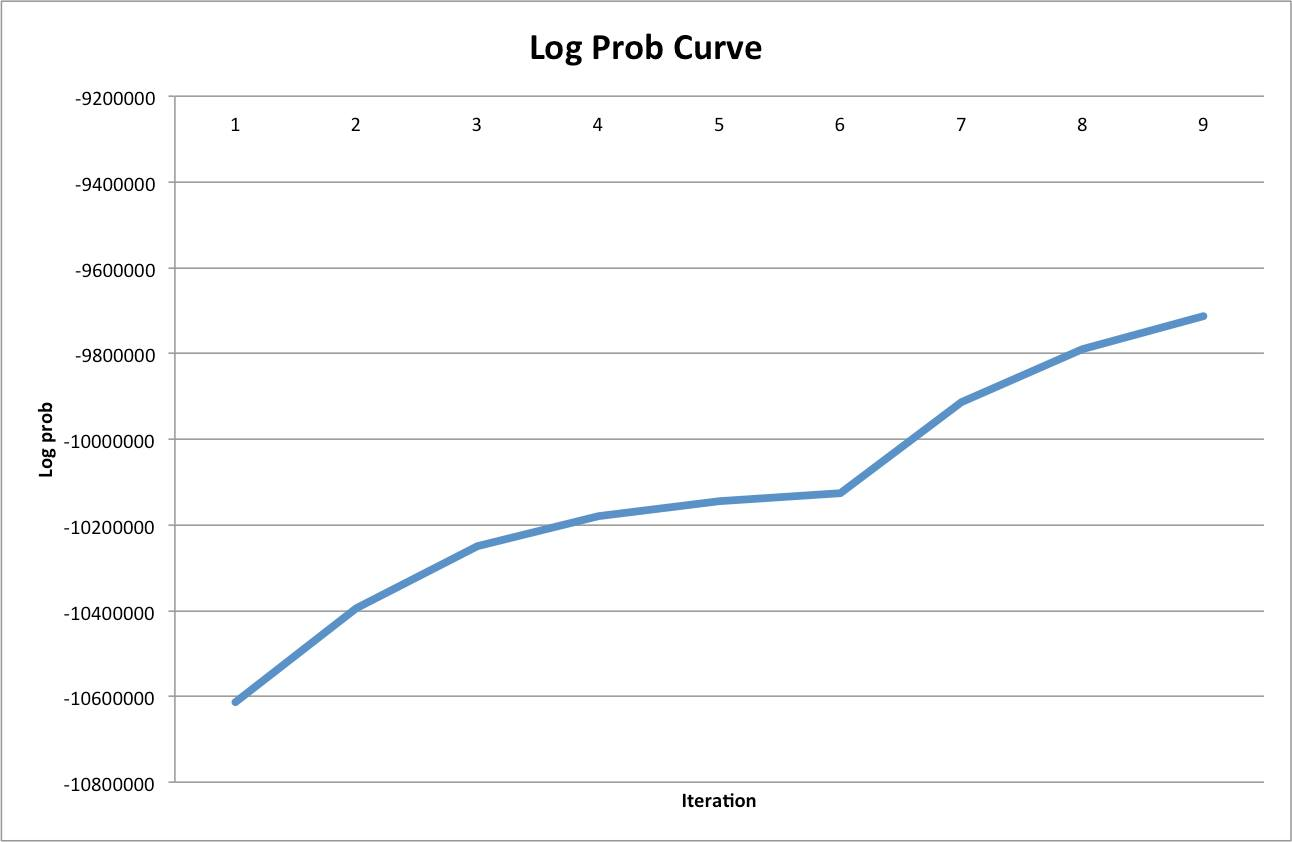
\includegraphics[width=220pt]{1.jpg}
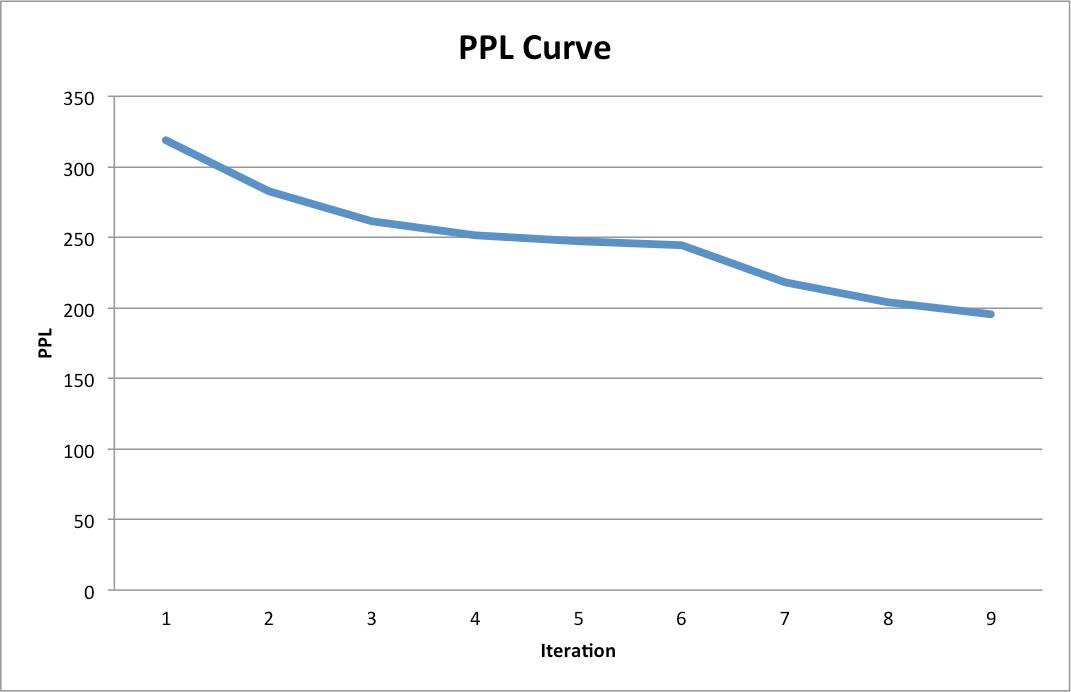
\includegraphics[width=220pt]{2.jpg}
\caption{The left figure (a) shows the log probability of RNNLM in each training iterations, and the right figure (b) shows the PPL in each iteration.}
\end{figure}
\section{Analysis and Comparison}
\subsection{Context Dependency}
N-gram and NNLM only consider the context dependency in the small window size of the sequence, while skip-gram consider larger and more flexible window size, and RNN considers the whole context history. In theory, more information considered, more powerful the model will be. But to our experiment result, N-gram is good enough to handle real tasks.
\subsection{Out of Vocabulary and word similarity}
Words in N-gram models are independent,They only map together identical words, but ignore similar or related words. While using meaningful vector representation, the other models can do better in OOV conditions. For example, if $P("\text{I am in Beijing}") =0 $, but the model knows "Beijing" is similar as "Taipei", and $P("\text{I am in Taipei}") >0 $, thus we can assign $P("\text{I am in Beijing}") >0 $.

According to Table 1 and 2, NN based model have better performance on OOV condition due to their vectorization strategy. 
\subsection{Training Speed}
N-gram without neural network train the model the fastest, and word2vec outperform the other NN models. NNLM and RNNLM take many hours to train one model. 
\subsection{Parameter Selection}
Because of their poor efficiency, NN models are difficult to do parameter selection. This was the biggest problem we met during the experiment. We haven't find a solution yet.
\subsection{Overfitting}
Since we didn't add regularization term, NNLM may have overfitted so that it failed to achieved the base accuracy 0.69.

In RNNLM experiment, as to model 2 it started to overfit after 11-hours training and the accurancy peaked at the ninth iteration. There are some reasons resulting in the problem. The first one is the sparse validation data. In order to speed up the training process, we have replaced the original validation data (22M) with the top 1k sentences (117kb), which, on the other way, leads to an early overfitting. The imperfect parameters may account for the second reason.There are more than 10 million words in the vocabulary and according to our former experiments, more than 200 hidden layers are needed to achieve a better result.

\section{Conclusion}
In conclusion, N-gram model with smoothing and backoff is useful in practice, but it cannot reveal the word similarity and hence can't deal with some OOV conditions. 
NN based model with good vector representation of words can handle more cases but it need well designed by parameter selections and speedups. Word2vec is quite efficient tool, but we haven't find a way to evaluate it in language model.
\section{Reference}
[1] https://en.wikipedia.org/wiki/N-gram \\ \ 
[2] Y. Bengio, R. Ducharme, P. Vincent. A neural probabilistic language model. Journal of Machine Learning Research, 3:1137-1155, 2003.\\ \
[3] Mikolov, T. (2012). Statistical language models based on neural networks. Presentation at Google, Mountain View, 2nd April.\\ \
[4] Mikolov, T., Chen, K., Corrado, G.,  Dean, J. (2013). Efficient estimation of word representations in vector space. arXiv preprint arXiv:1301.3781.\\ \
[5] https://code.google.com/p/word2vec/\\ \
[6] http://www.marekrei.com/teaching/lmtask\\ \
[7] http://www.speech.sri.com/projects/srilm/\\ \
[8] http://www.fit.vutbr.cz/~imikolov/rnnlm/\\ \
[9] https://en.wikipedia.org/wiki/Perplexity\\ \

\end{document}  